\documentclass[options]{article}
\usepackage[]{url}
\usepackage{graphicx}
\usepackage{hyperref}

\begin{document}
\title{Simulation of two interacting squirmers}
\author{Robin and Justine}
\date{May, 2024}
\maketitle

\section{Context}
Our project is part of the ANR project NEMO, Control of Magnetic Micro-swimmers in Complex and Confined Environments.
Currently, a team of researchers is developing numerical methods to control a micro-swimmer in the arteries
of the human body.
Ultimately, the goal of these robots is to treat cancer cells.

\vspace{0.5cm}
Our goal is to add Brumley's forces in the equation of the interactions between two squirmers, 
and afterward we will model it in a program. 
\begin{itemize}
    \item We also aim to investigate the effects of varying the distance between the squirmers to observe
    potential modifications in their behaviors.
    \item Furthermore, we plan to explore the impact of altering the parameter $\beta$, which defines the
    type of squirmers (pusher, puller, neutral), on their interactions.
    \item Additionally, we will conduct a comparative analysis between a squirming micro-robot and a 
    boundary. This analysis will involve varying the initial angle describing the micro-robot's 
    movement, the distance between the swimmer and the wall, as well as the parameter $\beta$, 
    to comprehensively understand their influence on the system dynamics.
\end{itemize}

\newpage
\section{Roadmap}
\begin{center}
    \href{https://github.com/orgs/master-csmi/projects/23/views/2}{Roadmap}
    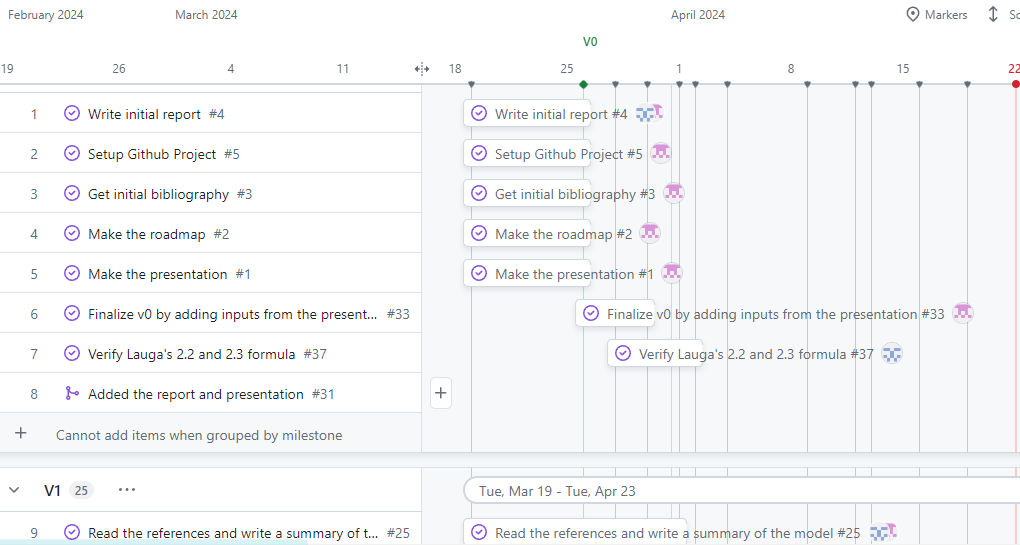
\includegraphics[width=0.9\textwidth]{V0/images/roadmapV0_1.png}
    \vspace{1em} % Ajoute un espace vertical
    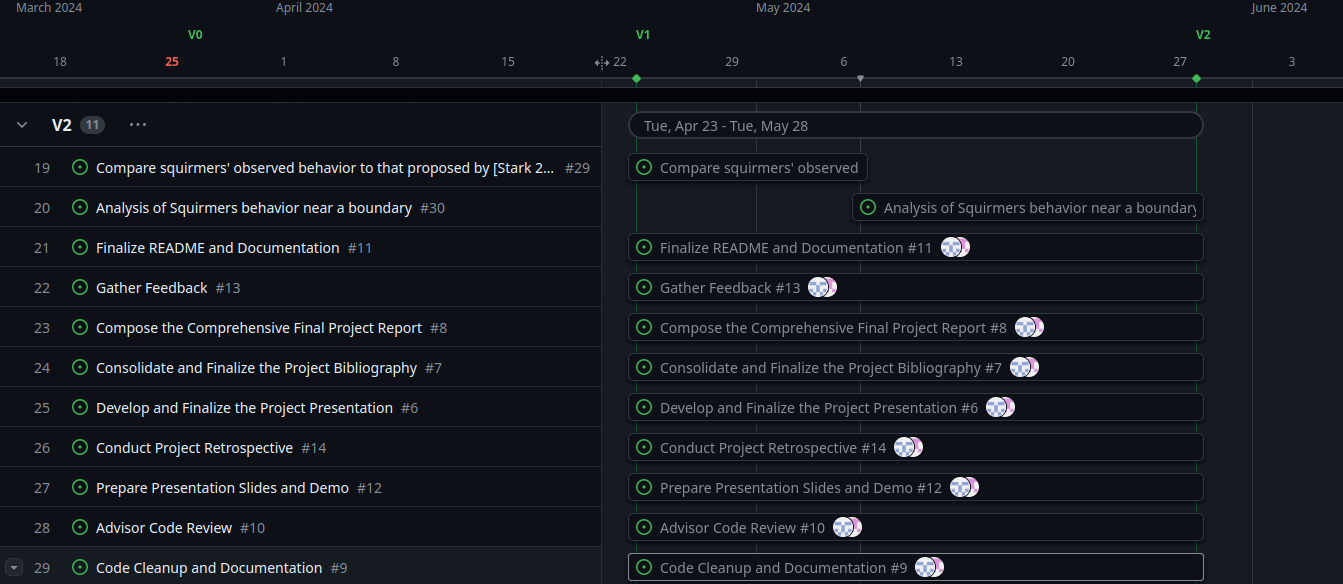
\includegraphics[width=0.9\textwidth]{V0/images/roadmapV0_2.png}
\end{center}


\nocite{*}
\bibliographystyle{plain}
\bibliography{V0/bibliography/biblio}
\end{document}